% !TeX encoding = UTF-8
% !TeX spellcheck = ru_RU

\section{Результаты}
\label{sec:Chapter4} \index{Chapter4}

\subsection{Характеристики устройства для тестов}

Перед обсуждением результатов, стоит привести характеристики устройства, использованного для тестирования реализованных методов:

\begin{itemize}
    \item CPU: 12th Gen Intel(R) Core(TM) i7-12650H
    \item Встроенное GPU: Intel(R) UHD Graphics
    \item Дискретное GPU: NVIDIA GeForce RTX 4070 Laptop GPU
    \item ОЗУ: 16GB
\end{itemize}
, где GPU - это графический процессор или видеокарта, а CPU - центральный процессор.

\subsection{Графическое API Vulkan}

Для рендеринга было выбрано графическое API \textit{Vulkan}, поскольку он является кроссплатформенным графическим API нового поколения (к новым относят \textit{DirectX 12}, \textit{Metal} и \textit{Vulkan}, к старым - \textit{OpenGL}, \textit{DirectX 11} и ниже), предоставляет более обширное управление для работы с видеокартой и обладает возможностью использования новых технологий последних лет (например сеточный шейдер (mesh shader) и трассировка лучей (ray tracing)).

\begin{figure}[h]
    \centering
    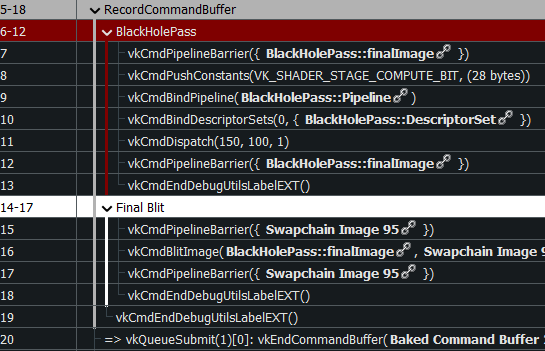
\includegraphics[width=0.8\linewidth]{CommandBuffer}
    \caption{Список команд, исполняющихся на GPU на каждом кадре. Получено при помощи приложения \textit{RenderDoc}.}
\end{figure}

Для всех методов используется \textit{Vulkan 1.0}, если не заявлено иначе. Все команды, исполняющиеся на GPU можно поделить на две группы:

\begin{enumerate}
    \item Визуализация черной дыры в вычислительном шейдере.
    \item Копирование вычисленного изображения в цепочку изображений \linebreak(swapchain) для последующего отображения на дисплей.
    \label{item:blit}
\end{enumerate}
, где вычислительный шейдер - аналог CUDA и OpenCL программ, исполняемых на GPU. Шаг \ref{item:blit} является крайне легковесным и почти не влияющим на производительность.

\begin{figure}[h]
    \centering
    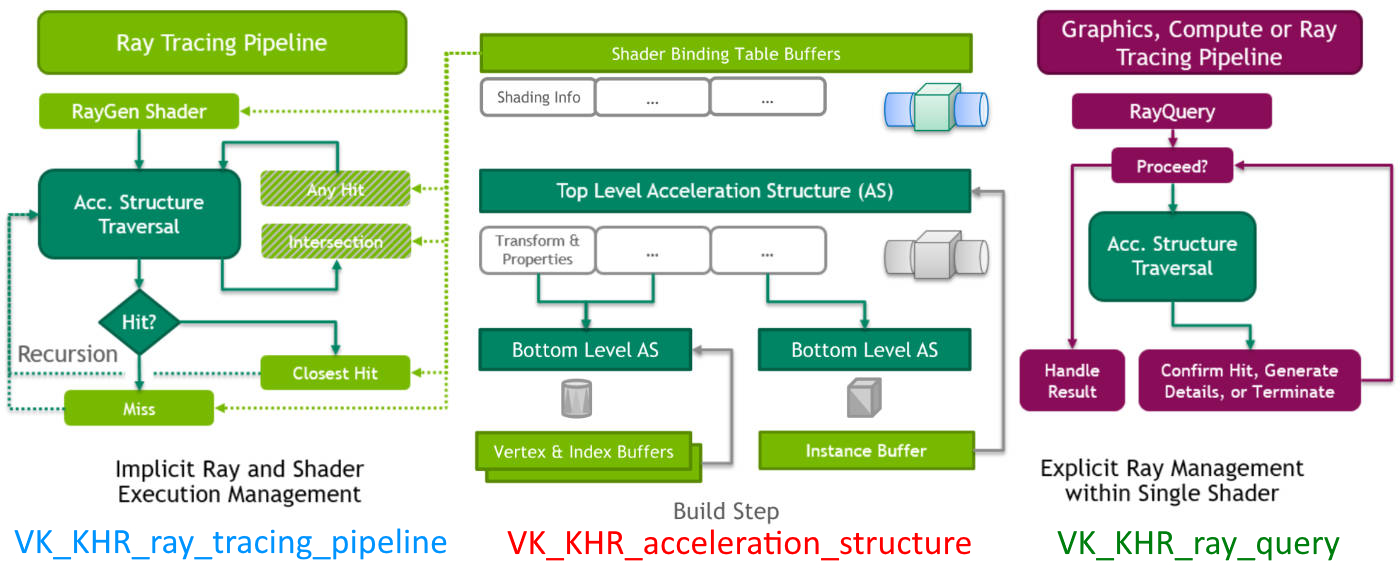
\includegraphics[width=1.0\linewidth]{Ray-Tracing-Overview}
    \caption{Набор расширений \textit{Vulkan Ray Tracing}.}
    \label{fig:raytracing_overview}
\end{figure}

При использовании трассировки лучей используется \textit{Vulkan 1.2} с набором расширений \textit{Ray Tracing} (см. рис. \ref{fig:raytracing_overview}): ускоряющие структуры\linebreak (acceleration structures), конвейер трассировки лучей (ray tracing pipeline) и запрос лучей (ray query). В работе используются первое и последнее расширения.

Ускоряющие структуры (acceleration structures) предоставляют скрытую реализацию иерархии ограничивающих объемов (bounding volume\linebreak hierarchy), чтобы совершать быстрый обход всей геометрии на сцене для поиска пересечения с лучем.

Запрос луча (ray query) нужен для самой трассировки лучей. Это расширение является альтернативой расширению конвейера трассировки лучей (ray tracing pipeline), но выделяет ее легкость использования, меньшая нагрузка на драйвер GPU, а также возможность использования в различных, в том числе фрагментных и \underline{вычислительных} шейдерах, что крайне полезно в случае данной работы.

\subsection{Сравнение реализованных методов}

\subsubsection{Визуальная составляющая}

Визуальный результат представлен на рисунках \ref{fig:black_hole_ray_marching}, \ref{fig:black_hole_precomputed} и \ref{fig:blackhole_raytracing}, а также в Приложении Б.

Если использовать реализацию марширования лучей (см. раздел \ref{sec:Chapter1}) для сравнения с другими, то в случае предвычисленных данных (см. раздел \ref{sec:Chapter2}) аккреционный диск превратился из трехмерного в двумерный объект, а в случае реализации комбинации марширования лучей и трассировки лучей - добавление новых объектов.

\subsubsection{Производительность}

Производительность будет измеряться в количестве \textbf{вычисленных}, а не отображенных на дисплее, кадров в секунду (frames per second, FPS). Разница существенная - количество отображенных кадров ограничено частотой обновления дисплея, а количество вычисленных кадров ограничено только мощностью устройства. Тем самым будет измеряться реальная производительность методов. В API \textit{Vulkan} это делается указанием \verb|VK_PRESENT_MODE_MAILBOX_KHR| при выборе режима представления цепочки изображений (swapchain).

Итак, результаты представлены ниже:

\begin{center}
    \begin{table}[h!]
        \centering
        \begin{tabular}{|c|cccccc|}
        \hline
        \multirow{3}{*}{GPU} & \multicolumn{6}{c|}{FPS}                                                                                                                                                                                                                      \\ \cline{2-7} 
                             & \multicolumn{2}{c|}{RK1}                                                             & \multicolumn{2}{c|}{RK2}                                                             & \multicolumn{2}{c|}{RK4}                                        \\ \cline{2-7} 
                             & \multicolumn{1}{c|}{$\Delta\phi = 0.003$} & \multicolumn{1}{c|}{$\Delta\phi = 0.01$} & \multicolumn{1}{c|}{$\Delta\phi = 0.003$} & \multicolumn{1}{c|}{$\Delta\phi = 0.01$} & \multicolumn{1}{c|}{$\Delta\phi = 0.003$} & $\Delta\phi = 0.01$ \\ \hline
        RTX 4070 Laptop      & \multicolumn{1}{c|}{190}                  & \multicolumn{1}{c|}{630}                 & \multicolumn{1}{c|}{175}                  & \multicolumn{1}{c|}{588}                 & \multicolumn{1}{c|}{141}                  & 470                 \\ \hline
        Intel UHD Graphics   & \multicolumn{1}{c|}{33}                   & \multicolumn{1}{c|}{100}                 & \multicolumn{1}{c|}{25}                   & \multicolumn{1}{c|}{79}                  & \multicolumn{1}{c|}{17}                   & 53                  \\ \hline
        \end{tabular}
        \caption{Производительность метода рендеринга черной дыры маршированием лучей (раздел \ref{subsec:algos}).}
        \label{tab:results_raymarching}
    \end{table}
\end{center}

Отчетливо видно падение производительности при увеличении порядка метода Рунге-Кутты, поскольку с увеличением порядка увеличивается и вычислительная сложность алгоритма. Также с уменьшением шага метода Рунге-Кутты $\Delta\phi$ также увеличивается производительность в связи с уменьшением количества итераций. Дополнительно следует отметить падение производительности при переходе с RTX 4070 Laptop на Intel UHD Graphics.

\begin{center}
    \begin{table}[h!]
        \centering
        \begin{tabular}{|c|c|}
        \hline
        GPU                & FPS  \\ \hline
        RTX 4070 Laptop    & 9950 \\ \hline
        Intel UHD Graphics & 330  \\ \hline
        \end{tabular}
        \caption{Производительность метода рендеринга черной дыры при помощи предрасчитанных данных (раздел \ref{subsec:precompute_black_hole_rendering}).}
        \label{tab:results_precomputed}
    \end{table}
\end{center}

Наблюдается прирост FPS в десятки раз в случае использования предрасчитанных данных по сравнению с маршированием лучей. Однако за такой прирост необходимо платить большим использованием видеопямяти для хранения предрасчитанных данных (например в данной работе для трехмерной текстуры предрассчитанных данных аккреционного диска размером $(640, 640, 128)$ и содержащем в каждом своем пикселе по два значения типа \textit{float32} (IEEE-754) занятый объем видеопамяти составляет примерно 400 мегабайт).

\begin{center}
    \begin{table}[h!]
        \centering
        \begin{tabular}{|c|cc|}
        \hline
        \multirow{3}{*}{GPU} & \multicolumn{2}{c|}{FPS}                                        \\ \cline{2-3} 
                             & \multicolumn{2}{c|}{RK1}                                        \\ \cline{2-3} 
                             & \multicolumn{1}{c|}{$\Delta\phi = 0.003$} & $\Delta\phi = 0.01$ \\ \hline
        RTX 4070 Laptop      & \multicolumn{1}{c|}{18}                   & 60                  \\ \hline
        \end{tabular}
        \caption{Производительность метода рендеринга черной дыры комбинацией марширования лучей и трассировки лучей (раздел \ref{subsec:new_algos}).}
        \label{tab:results_raymarchingtracing}
    \end{table}
\end{center}

Использование трассировки лучей очень сильно влияет на производительность, поскольку она используется на каждой итерации. Поэтому наблюдается падение производительности по сравнению с обычным маршированием лучей в примерно десять раз.

\newpage